
\tikzset{every picture/.style={line width=0.75pt}}
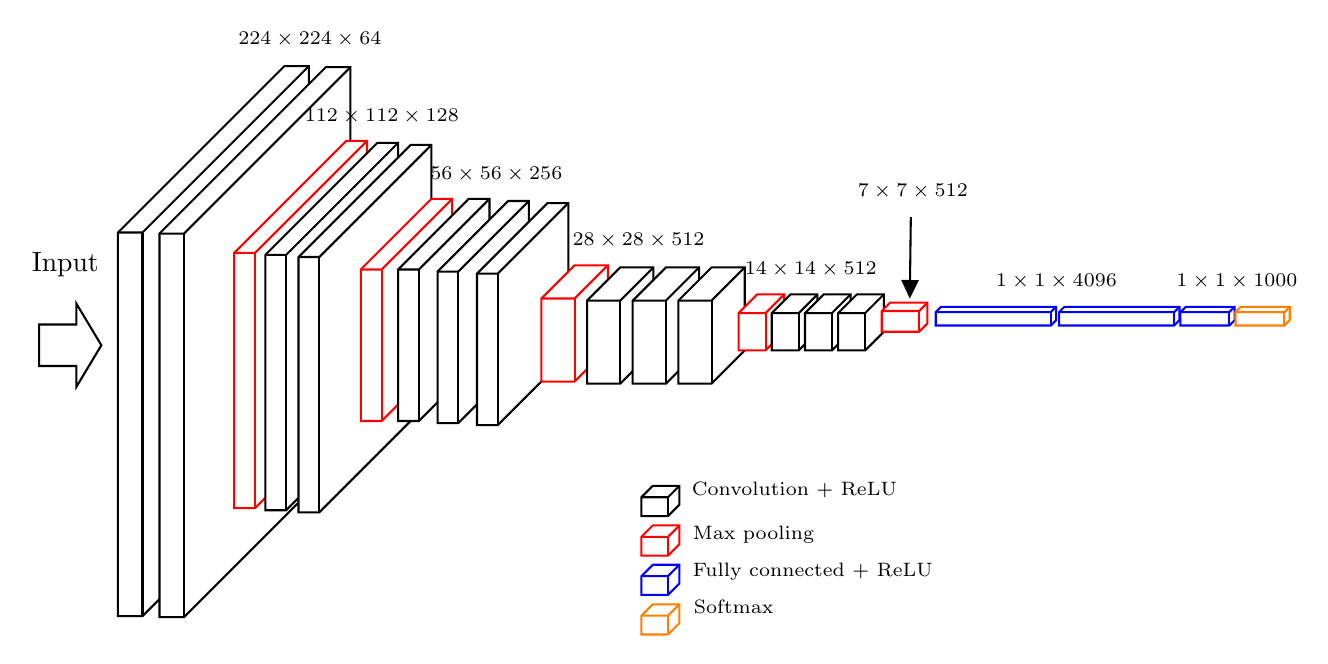
\begin{tikzpicture}[x=0.75pt,y=0.75pt,yscale=-1,xscale=1]

% Conv1-1 
\draw  [fill=white  ,fill opacity=1 ] (44,95.69) -- (124.19,15.5) -- (136,15.5) -- (136,200.31) -- (55.81,280.5) -- (44,280.5) -- cycle ; \draw   (136,15.5) -- (55.81,95.69) -- (44,95.69) ; \draw   (55.81,95.69) -- (55.81,280.5) ;
% Conv 1-2
\draw  [fill=white  ,fill opacity=1 ] (64,96.19) -- (144.19,16) -- (156,16) -- (156,200.81) -- (75.81,281) -- (64,281) -- cycle ; \draw   (156,16) -- (75.81,96.19) -- (64,96.19) ; \draw   (75.81,96.19) -- (75.81,281) ;
% Pooling 1
\draw  [color=red  ,draw opacity=1 ][fill=white  ,fill opacity=1 ] (100,105.5) -- (154,51.5) -- (164,51.5) -- (164,174.5) -- (110,228.5) -- (100,228.5) -- cycle ; \draw  [color=red  ,draw opacity=1 ] (164,51.5) -- (110,105.5) -- (100,105.5) ; \draw  [color=red  ,draw opacity=1 ] (110,105.5) -- (110,228.5) ;
% Conv 2-1
\draw  [fill=white  ,fill opacity=1 ] (115,106.5) -- (169,52.5) -- (179,52.5) -- (179,175.5) -- (125,229.5) -- (115,229.5) -- cycle ; \draw  [color={rgb, 255:red, 0; green, 0; blue, 0 }  ,draw opacity=1 ] (179,52.5) -- (125,106.5) -- (115,106.5) ; \draw  [color={rgb, 255:red, 0; green, 0; blue, 0 }  ,draw opacity=1 ] (125,106.5) -- (125,229.5) ;
% Conv 2-2
\draw  [fill=white  ,fill opacity=1 ] (131,107.5) -- (185,53.5) -- (195,53.5) -- (195,176.5) -- (141,230.5) -- (131,230.5) -- cycle ; \draw  [color={rgb, 255:red, 0; green, 0; blue, 0 }  ,draw opacity=1 ] (195,53.5) -- (141,107.5) -- (131,107.5) ; \draw  [color={rgb, 255:red, 0; green, 0; blue, 0 }  ,draw opacity=1 ] (141,107.5) -- (141,230.5) ;
% Pooling 2
\draw  [color=red  ,draw opacity=1 ][fill=white  ,fill opacity=1 ] (161,113.5) -- (195,79.5) -- (205,79.5) -- (205,152.5) -- (171,186.5) -- (161,186.5) -- cycle ; \draw  [color=red  ,draw opacity=1 ] (205,79.5) -- (171,113.5) -- (161,113.5) ; \draw  [color=red  ,draw opacity=1 ] (171,113.5) -- (171,186.5) ;
% Conv 3-1
\draw  [fill=white  ,fill opacity=1 ] (179,113.5) -- (213,79.5) -- (223,79.5) -- (223,152.5) -- (189,186.5) -- (179,186.5) -- cycle ; \draw  [color={rgb, 255:red, 0; green, 0; blue, 0 }  ,draw opacity=1 ] (223,79.5) -- (189,113.5) -- (179,113.5) ; \draw  [color={rgb, 255:red, 0; green, 0; blue, 0 }  ,draw opacity=1 ] (189,113.5) -- (189,186.5) ;
% Conv 3-2
\draw  [fill=white  ,fill opacity=1 ] (198,114.5) -- (232,80.5) -- (242,80.5) -- (242,153.5) -- (208,187.5) -- (198,187.5) -- cycle ; \draw  [color={rgb, 255:red, 0; green, 0; blue, 0 }  ,draw opacity=1 ] (242,80.5) -- (208,114.5) -- (198,114.5) ; \draw  [color={rgb, 255:red, 0; green, 0; blue, 0 }  ,draw opacity=1 ] (208,114.5) -- (208,187.5) ;
% Conv 3-3
\draw  [fill=white  ,fill opacity=1 ] (217,115.5) -- (251,81.5) -- (261,81.5) -- (261,154.5) -- (227,188.5) -- (217,188.5) -- cycle ; \draw  [color={rgb, 255:red, 0; green, 0; blue, 0 }  ,draw opacity=1 ] (261,81.5) -- (227,115.5) -- (217,115.5) ; \draw  [color={rgb, 255:red, 0; green, 0; blue, 0 }  ,draw opacity=1 ] (227,115.5) -- (227,188.5) ;
% Pooling 3
\draw  [color=red  ,draw opacity=1 ][fill=white  ,fill opacity=1 ] (248,127.5) -- (264,111.5) -- (280,111.5) -- (280,151.5) -- (264,167.5) -- (248,167.5) -- cycle ; \draw  [color=red  ,draw opacity=1 ] (280,111.5) -- (264,127.5) -- (248,127.5) ; \draw  [color=red  ,draw opacity=1 ] (264,127.5) -- (264,167.5) ;
% Conv 4-1
\draw  [fill=white  ,fill opacity=1 ] (270,128.5) -- (286,112.5) -- (302,112.5) -- (302,152.5) -- (286,168.5) -- (270,168.5) -- cycle ; \draw  [color={rgb, 255:red, 0; green, 0; blue, 0 }  ,draw opacity=1 ] (302,112.5) -- (286,128.5) -- (270,128.5) ; \draw  [color={rgb, 255:red, 0; green, 0; blue, 0 }  ,draw opacity=1 ] (286,128.5) -- (286,168.5) ;
% Conv 4-2
\draw  [fill=white  ,fill opacity=1 ] (292,128.5) -- (308,112.5) -- (324,112.5) -- (324,152.5) -- (308,168.5) -- (292,168.5) -- cycle ; \draw  [color={rgb, 255:red, 0; green, 0; blue, 0 }  ,draw opacity=1 ] (324,112.5) -- (308,128.5) -- (292,128.5) ; \draw  [color={rgb, 255:red, 0; green, 0; blue, 0 }  ,draw opacity=1 ] (308,128.5) -- (308,168.5) ;
% Conv 4-3
\draw  [fill=white  ,fill opacity=1 ] (314,128.5) -- (330,112.5) -- (346,112.5) -- (346,152.5) -- (330,168.5) -- (314,168.5) -- cycle ; \draw  [color={rgb, 255:red, 0; green, 0; blue, 0 }  ,draw opacity=1 ] (346,112.5) -- (330,128.5) -- (314,128.5) ; \draw  [color={rgb, 255:red, 0; green, 0; blue, 0 }  ,draw opacity=1 ] (330,128.5) -- (330,168.5) ;
% pooling 4
\draw  [color=red  ,draw opacity=1 ][fill=white  ,fill opacity=1 ] (343,134.5) -- (352,125.5) -- (365,125.5) -- (365,143.5) -- (356,152.5) -- (343,152.5) -- cycle ; \draw  [color={rgb, 255:red, 251; green, 0; blue, 0 }  ,draw opacity=1 ] (365,125.5) -- (356,134.5) -- (343,134.5) ; \draw  [color={rgb, 255:red, 251; green, 0; blue, 0 }  ,draw opacity=1 ] (356,134.5) -- (356,152.5) ;
% Conv 5-1
\draw  [fill=white  ,fill opacity=1 ] (359,134.5) -- (368,125.5) -- (381,125.5) -- (381,143.5) -- (372,152.5) -- (359,152.5) -- cycle ; \draw  [color={rgb, 255:red, 0; green, 0; blue, 0 }  ,draw opacity=1 ] (381,125.5) -- (372,134.5) -- (359,134.5) ; \draw  [color={rgb, 255:red, 0; green, 0; blue, 0 }  ,draw opacity=1 ] (372,134.5) -- (372,152.5) ;
% Conv 5-2
\draw  [fill=white  ,fill opacity=1 ] (375,134.5) -- (384,125.5) -- (397,125.5) -- (397,143.5) -- (388,152.5) -- (375,152.5) -- cycle ; \draw  [color={rgb, 255:red, 0; green, 0; blue, 0 }  ,draw opacity=1 ] (397,125.5) -- (388,134.5) -- (375,134.5) ; \draw  [color={rgb, 255:red, 0; green, 0; blue, 0 }  ,draw opacity=1 ] (388,134.5) -- (388,152.5) ;
% COnv 5-3
\draw  [fill=white  ,fill opacity=1 ] (391,134.5) -- (400,125.5) -- (413,125.5) -- (413,143.5) -- (404,152.5) -- (391,152.5) -- cycle ; \draw  [color={rgb, 255:red, 0; green, 0; blue, 0 }  ,draw opacity=1 ] (413,125.5) -- (404,134.5) -- (391,134.5) ; \draw  [color={rgb, 255:red, 0; green, 0; blue, 0 }  ,draw opacity=1 ] (404,134.5) -- (404,152.5) ;
% Pooling 5
\draw  [color=red  ,draw opacity=1 ][fill=white  ,fill opacity=1 ] (412,133.5) -- (416,129.5) -- (434,129.5) -- (434,139.5) -- (430,143.5) -- (412,143.5) -- cycle ; \draw  [color=red  ,draw opacity=1 ] (434,129.5) -- (430,133.5) -- (412,133.5) ; \draw  [color=red  ,draw opacity=1 ] (430,133.5) -- (430,143.5) ;
% dense 1
\draw  [color=blue  ,draw opacity=1 ][fill=white  ,fill opacity=1 ] (438,134.07) -- (440.57,131.5) -- (496,131.5) -- (496,137.93) -- (493.43,140.5) -- (438,140.5) -- cycle ; \draw  [color=blue  ,draw opacity=1 ] (496,131.5) -- (493.43,134.07) -- (438,134.07) ; \draw  [color=blue  ,draw opacity=1 ] (493.43,134.07) -- (493.43,140.5) ;
% dense 2
\draw  [color=blue  ,draw opacity=1 ][fill=white  ,fill opacity=1 ] (497.43,134.07) -- (500,131.5) -- (555.43,131.5) -- (555.43,137.93) -- (552.86,140.5) -- (497.43,140.5) -- cycle ; \draw  [color=blue  ,draw opacity=1 ] (555.43,131.5) -- (552.86,134.07) -- (497.43,134.07) ; \draw  [color=blue  ,draw opacity=1 ] (552.86,134.07) -- (552.86,140.5) ;
% dense 3
\draw  [color=blue  ,draw opacity=1 ][fill=white  ,fill opacity=1 ] (555.86,134.07) -- (558.43,131.5) -- (582,131.5) -- (582,137.93) -- (579.43,140.5) -- (555.86,140.5) -- cycle ; \draw  [color=blue  ,draw opacity=1 ] (582,131.5) -- (579.43,134.07) -- (555.86,134.07) ; \draw  [color=blue  ,draw opacity=1 ] (579.43,134.07) -- (579.43,140.5) ;
% softmax
\draw  [color=orange  ,draw opacity=1 ][fill=white  ,fill opacity=1 ] (582.43,134.07) -- (585,131.5) -- (608.57,131.5) -- (608.57,137.93) -- (606,140.5) -- (582.43,140.5) -- cycle ; \draw  [color=orange  ,draw opacity=1 ] (608.57,131.5) -- (606,134.07) -- (582.43,134.07) ; \draw  [color=orange  ,draw opacity=1 ] (606,134.07) -- (606,140.5) ;
% input
\draw   (6,140) -- (24,140) -- (24,130) -- (36,150) -- (24,170) -- (24,160) -- (6,160) -- cycle ;
% arrow
\draw    (426,88.25) -- (425.54,124.5) ;
\draw [shift={(425.5,127.5)}, rotate = 270.73] [fill={rgb, 255:red, 0; green, 0; blue, 0 }  ][line width=0.08]  [draw opacity=0] (8.93,-4.29) -- (0,0) -- (8.93,4.29) -- cycle    ;
% conv
\draw  [fill=white  ,fill opacity=1 ] (296.19,223.25) -- (301.69,217.75) -- (314.5,217.75) -- (314.5,226.81) -- (309,232.31) -- (296.19,232.31) -- cycle ; \draw   (314.5,217.75) -- (309,223.25) -- (296.19,223.25) ; \draw   (309,223.25) -- (309,232.31) ;
% max pool
\draw  [color=red  ,draw opacity=1 ][fill=white  ,fill opacity=1 ] (296.19,242.31) -- (301.69,236.81) -- (314.5,236.81) -- (314.5,245.87) -- (309,251.37) -- (296.19,251.37) -- cycle ; \draw  [color=red  ,draw opacity=1 ] (314.5,236.81) -- (309,242.31) -- (296.19,242.31) ; \draw  [color=red  ,draw opacity=1 ] (309,242.31) -- (309,251.37) ;
% fully connected
\draw  [color=blue  ,draw opacity=1 ][fill=white  ,fill opacity=1 ] (296.19,261.25) -- (301.69,255.75) -- (314.5,255.75) -- (314.5,264.81) -- (309,270.31) -- (296.19,270.31) -- cycle ; \draw  [color=blue  ,draw opacity=1 ] (314.5,255.75) -- (309,261.25) -- (296.19,261.25) ; \draw  [color=blue  ,draw opacity=1 ] (309,261.25) -- (309,270.31) ;
% softmax
\draw  [color=orange  ,draw opacity=1 ][fill=white  ,fill opacity=1 ] (296.19,280.31) -- (301.69,274.81) -- (314.5,274.81) -- (314.5,283.87) -- (309,289.37) -- (296.19,289.37) -- cycle ; \draw  [color=orange  ,draw opacity=1 ] (314.5,274.81) -- (309,280.31) -- (296.19,280.31) ; \draw  [color=orange  ,draw opacity=1 ] (309,280.31) -- (309,289.37) ;

 
\draw (1,104) node [anchor=north west][inner sep=0.75pt]   [align=left] {Input};
 
\draw (100.5,-2.5) node [anchor=north west][inner sep=0.75pt]  [font=\scriptsize]  {$224\times 224\times 64$};
 
\draw (132.5,34.5) node [anchor=north west][inner sep=0.75pt]  [font=\scriptsize]  {$112\times 112\times 128$};
 
\draw (261.5,94.5) node [anchor=north west][inner sep=0.75pt]  [font=\scriptsize]  {$28\times 28\times 512$};
 
\draw (344.5,108.5) node [anchor=north west][inner sep=0.75pt]  [font=\scriptsize]  {$14\times 14\times 512$};
 
\draw (193,62.5) node [anchor=north west][inner sep=0.75pt]  [font=\scriptsize]  {$56\times 56\times 256$};

\draw (399,71) node [anchor=north west][inner sep=0.75pt]  [font=\scriptsize]  {$7\times 7\times 512$};

\draw (465.5,114) node [anchor=north west][inner sep=0.75pt]  [font=\scriptsize]  {$1\times 1\times 4096$};

\draw (552.5,114) node [anchor=north west][inner sep=0.75pt]  [font=\scriptsize]  {$1\times 1\times 1000$};


\draw (319,214.5) node [anchor=north west][inner sep=0.75pt]  [font=\scriptsize] [align=left] {Convolution + ReLU};

\draw (319.5,235.5) node [anchor=north west][inner sep=0.75pt]  [font=\scriptsize] [align=left] {Max pooling};

\draw (319.5,253.5) node [anchor=north west][inner sep=0.75pt]  [font=\scriptsize] [align=left] {Fully connected + ReLU};

\draw (320,271.5) node [anchor=north west][inner sep=0.75pt]  [font=\scriptsize] [align=left] {Softmax};


\end{tikzpicture}
